% !TEX root=../../Thesis.tex
\chapter{Generalizing over different scenarios} \label{ch:generalize}
% \tommy{Uncertainty in MDP which one are we in?}
% \begin{center}
%   \textit{\textbf{RQ 3: How can a \gls{rl} agent handle situations it has not been trained on?}}
%   \end{center}
%   \vspace{12pt}

% As mentioned in the Seciton \ref{sec:background_mdp}. The \gls{mdp} is defined by the tuple (S,A,R,T,$\gamma$). The work until now has solved the \gls{mdp} or \gls{pomdp} without defining the transition function T by using \gls{rl}. 
% So what happens when you take a policy trained on one \gls{mdp} defined by one transition function T1 and put it in another simulation with transition funciton T2? Well the short answer is that because \gls{dqn} uses a \gls{nn} to approximate the utility Q for taking an action in each state. 

% A transition function T is defined as the probability of transitioning from one state to another. The transition function could be different for example when the ego vehicle properties are different, if the \gls{dqn} is trained on a sports car and then applied on a truck, the difference in acceleration capability would result in a different transition function. Another example would be on the other traffic participants, if the \gls{dqn} is trained in an environment where the driving culture is on the passive side and that is later put in an environment that has a more aggressive driving culture. The \gls{dqn} would probably not perform so well. 
% This is especially important when you have an intention state directly correlated with the transition. For example in \paperD were the intentions are described on a high level such as take way or give way. 
% An example is lane changes in Sweden, it is normal to signal first, wait for the other vehicle to slow down before initiating a lane change. While in a high density traffic jam in Paris, it is more normal to show intention by starting a lane change and observe if the other vehicle yields. 

In the previous chapter, the experiments demonstrated how an agent can utilize the uncertainty measurement to reduce the number of collisions. This chapter explores how to identify when an agent is acting in a scenario outside its training set.

Let's consider that a company is designing Level 5 \gls{ad} agents. As mentioned in Section~\ref{sec:intro_ad}, L5 requires the \gls{av} to be able to drive anywhere. The company has already designed two RL agents that have learned to drive at L4 in the USA and UK. Now, the company wants to deploy a new \gls{rl} agent in India. 
Though all the \gls{rl} agents are concerned with the same task, i.e. driving, the models encompassing driver behaviors, traffic rules, signs, etc., can differ for each. For example, UK and India have left-handed traffic, while the USA has right-handed traffic. However, learning a new controller specifically for every new geographic location is computationally expensive and time-consuming, as both data collection and learning take time. Thus, the company might use the models learned for UK and USA, to estimate the model for India, and use it further to build a new \gls{rl} agent. Hence, being able to transfer the source models to the target environment allows the company to use existing knowledge to build a new agent faster while using less resources. 
This problem of model transfer from source models to a target environment to plan efficiently is address in \paperTransfer. 

\section{Approach}
In this example, the driving model for each country is defined by its own \gls{mdp}. A set of source \gls{mdp}s $\mathcal{M}_s \triangleq \{\mu_i\}_{i=1}^m$ is used to create a convex hull of \gls{mdp}s $\mathcal{C}(\mathcal{M}_s)$, where each \gls{mdp} $\mu_i$ acts as a boundary. 
The proposed approach, Maximum Likelihood Estimation for Model-based Transfer RL (MLEMTRL), involves using model transfer \gls{rl} to determine the unknown target \gls{mdp}s $\mu^* \in \mathcal{C}(\mathcal{M}_s)$ position within this convex hull of \gls{mdp}s and then find an optimal policy $\pi^*$ for that \gls{mdp}. 
This method relies on having a diverse set of \gls{mdp}s to effectively span the convex hull of models, thereby facilitating the discovery of optimal policies between \gls{mdp}s. For example, downtown driving behavior in one country may closely resemble that in another. For the case when $\mu^*$ is close but outside $\mathcal{C}(\mathcal{M}_s)$, see \paperTransfer.

% \todo{cons: computationally heavy. Have to create the complex hull of MDPs from e set of MDPs.}
% \todo{Pros: able to identify which policy to use and scale better by generalizing MDPs instead of countries.}


\begin{algorithm}[t!]
  \caption{Maximum Likelihood Estimation for Model-based Transfer RL (MLEMTRL)}\label{alg:thesis_mlemtrl}
  \begin{algorithmic}[1]
  \State \textbf{Input:} weights $\bm{w}^0$, $m$ source MDPs $\mathcal{M}_s$, data $D_0$, discount factor $\gamma$, iterations $T$.
  \For{$t=0, \hdots, T$}
  \State\textsc{// Stage 1: Model Estimation //}
  \State $\bm{w}^{t+1}\leftarrow  \textsc{Optimiser}(\log\mathbb{P}(D_t \, | \, \Sigma_{i=1}^m w_i \mu_i), \bm{w}^t)$
  \State Estimate the MDP: $\mu^{t+1} = \sum_{i=1}^m w_i \mu_i$
  \State\textsc{// Stage 2: Model-based Planning //}
  \State Compute the policy: $\pi^{t+1} \in \underset{\pi}{\arg\max} \, V_{\mu^{t+1}}^\pi$
  \State\textsc{// Control //}
  \State Observe $s_{t+1}, r_{t+1} \sim \mu^{*}(s_t, a_t), a_t\sim \pi^{t+1}(s_t)$
  \State Update the dataset $D_{t+1} = D_t \cup \{s_t, a_t, s_{t+1}, r_{t+1}\}$
  \EndFor
  \State \textbf{return} An estimated MDP model $\mu^T$ and a policy $\pi^T$
  \end{algorithmic}
\end{algorithm}

The MLEMTRL algorithm, outlined in Algorithm~\ref{alg:thesis_mlemtrl}, consists of a \textit{model estimation} stage and a \textit{planning} stage. 

\noindent\textbf{Model estimation:} This stage estimates a \gls{mdp} $\hat{\mu}$ from a compact subset of $m$ source \gls{mdp}s, $\mu' \subset \mathcal{M}_s$, utilizing data from experience $D_t$ gathered by taking actions in the environment.
Let's define the convex hull as $\mathcal{C}(\mathcal{M}_s) \triangleq \{\mu_1 w_1 + \hdots + \mu_m w_m \, | \, \mu_i \in \mathcal{M}_s, w_i \geq 0, i=1, \hdots, m, \sum_{i=1}^m w_i = 1\}$. Then, the corresponding MLE problem with the corresponding likelihood function is
\begin{equation}\label{eq:thesis_realisable}
    \hat{\mu} \in \underset{\mu' \in \mathcal{C}(\mathcal{M}_s)}{\arg\max} \, \log \mathbb{P}(D_t \, | \, \mu'), D_t \sim \mu^{*}.
\end{equation}
Since $\mathcal{C}(\mathcal{M}_s)$ induces a compact subset of model parameters $\mathcal{M}' \subset \mathcal{M}$, \eqref{eq:thesis_realisable} leads to a constrained maximum likelihood estimation problem~\citep{aitchison1958maximum}. It implies that if the parameter corresponding to the target \gls{mdp} is in $\mathcal{M}'$, it can be correctly identified.
For continuous state-action MDPs, a linear-Gaussian likelihood is used. In this context, let $d_s$ be the dimensionality of the state-space, $\bm{s} \in \mathbb{R}^{d_s}$ and $d_a$ be the dimensionality of the action-space. Then, the mean function $\mathbf{M}$ is a $\mathbb{R}^{d_s}\times\mathbb{R}^{d_a+d_s}$ matrix. The mean visitation count to the successor state $\bm{s}_t'$ when an action $\bm{a}_t$ is taken at state $\bm{s}_t$ is given by $\mathbf{M}(\bm{a}_t, \bm{s}_t)$. The corresponding covariance matrix, denoted by $\mathbf{S}$, is of size $\mathbb{R}^{d_s}\times\mathbb{R}^{d_s}$. The log-likelihood is then expressed as follows:
\begin{align*}
\begin{aligned}
    \log \mathbb{P}(D_t \, | \, \mathbf{M}, \mathbf{S}) &= \log \prod_{i=1}^t \frac{\exp\Big(-\frac{1}{2}\bm{v}^\top\mathbf{S}^{-1}\bm{v}\Big)}{(2\pi)^{d_s/2}|\mathbf{S}|^{1/2}},\\
    &\textrm{where} \,  \bm{v} = \bm{s}_i'-\mathbf{M}(\bm{a}_i, \bm{s}_i).
\end{aligned}
\end{align*}

As the optimization problem involves weighing multiple source models together, a weight vector $\bm{w} \in [0, 1]^{m}$ is introduced, with the usual property that $\bm{w}$ sum to $1$. 
% This addition results in another outer product over the likelihoods shown above. 

\begin{equation}\label{eq:thesis_constrained_likelihood}
\begin{aligned}
\underset{\bm{w}}{\min} \quad &\log \mathbb{P}(D_t \, | \, \Sigma_{i=1}^m w_i \mu_i), D_t \sim \mu^{*}, \mu_i\in\mathcal{M}_s,\\
\textrm{s.t.} \quad & \sum_{i=1}^m w_i = 1, w_i\geq0.\\
\end{aligned}
\end{equation}

Because of the constraint on $\bm{w}$, this is a constrained nonlinear optimization problem. Any optimizer algorithm, denoted by \textsc{Optimizer}, can be used for this purpose.
When an appropriate model $\mu^{t+1}$ has been identified at time step $t$, the next stage of the algorithm involves model-based planning in the estimated MDP.

\noindent\textbf{Planning:}
This stage computes the policy $\pi^{t+1}$ that maximizes the expected reward given the value function $V_{\mu^{t+1}}^\pi$ based on $\mu^{t+1}$. 
After computing $\pi^{t+1}$, the agent executes actions in the environment to acquire new experiences $D_{t+1}$. These steps are repeated $T$ times before producing a final estimated \gls{mdp} model $\mu^T$ and a policy $\pi^T$ is given.

Given the model, $\mu^t$ and the associated reward function $\mathcal{R}$, the optimal value function of $\mu^t$ can be computed iteratively as~\citep{Sutton2018}:
\begin{equation}\label{eq:thesis_value_iteration}
    V_{\mu^t}^{*}(s) = \underset{a}{\max} \, \sum_{s'}\mathcal{T}_{s,s'}^a\Big(\mathcal{R}(s,a)+\gamma V_{\mu^t}^{*}(s')\Big).
\end{equation}
The fixed-point solution to Eq.~\eqref{eq:thesis_value_iteration} is the optimal value function, where $\mathcal{T}$ is the transition function introduced in Section.~\ref{sec:pomdp_transistionmodel}. When the optimal value function has been obtained, one can simply select the action maximizing the action-value function. Let $\pi^{t+1}$ be the policy selecting the maximizing action for every state, then $\pi^{t+1}$ is the policy the model-based planner will use at time step $t+1$.

% For completeness, an extension to MLEMTRL called Meta-MLEMLTRL is also provided in \paperTransfer. This extension combines the MLEMTRL estimated model with the empirical model of the target task. This allows us to identify the true model even in the non-realisable setting.

% \begin{figure}
%   \center
%   % This file was created with tikzplotlib v0.10.1.
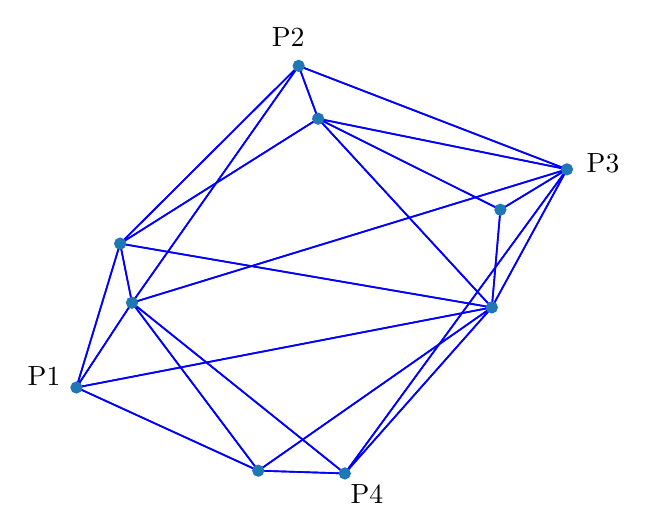
\begin{tikzpicture}

\definecolor{darkgray176}{RGB}{176,176,176}
\definecolor{steelblue31119180}{RGB}{31,119,180}

\begin{axis}[
hide x axis,
hide y axis,
tick align=outside,
tick pos=left,
x grid style={darkgray176},
xmin=0.0830648048633814, xmax=1.01851592807339,
xtick style={color=black},
y grid style={darkgray176},
ymin=-0.0194663712213591, ymax=0.936395207946179,
ytick style={color=black},
yticklabel style={anchor=center}
]
\addplot [draw=steelblue31119180, fill=steelblue31119180, mark=*, only marks]
table{%
x  y
0.510827605197663 0.892946954347655
0.125585310463836 0.207242878138187
0.440809843650636 0.029876210878567
0.590862817416351 0.0239818823771654
0.544649018031845 0.780314764511367
0.221957883932181 0.387971257555649
0.975995422472934 0.672383675912814
0.845750871293179 0.377994041328889
0.860533912946926 0.586252904467821
0.201378711043073 0.514035059817442
};
\addplot [semithick, blue]
table {%
0.221957883932181 0.387971257555649
0.510827605197663 0.892946954347655
0.975995422472934 0.672383675912814
0.221957883932181 0.387971257555649
};
\addplot [semithick, blue]
table {%
0.590862817416351 0.0239818823771654
0.221957883932181 0.387971257555649
0.975995422472934 0.672383675912814
0.590862817416351 0.0239818823771654
};
\addplot [semithick, blue]
table {%
0.544649018031845 0.780314764511367
0.510827605197663 0.892946954347655
0.975995422472934 0.672383675912814
0.544649018031845 0.780314764511367
};
\addplot [semithick, blue]
table {%
0.440809843650636 0.029876210878567
0.221957883932181 0.387971257555649
0.125585310463836 0.207242878138187
0.440809843650636 0.029876210878567
};
\addplot [semithick, blue]
table {%
0.440809843650636 0.029876210878567
0.590862817416351 0.0239818823771654
0.221957883932181 0.387971257555649
0.440809843650636 0.029876210878567
};
\addplot [semithick, blue]
table {%
0.201378711043073 0.514035059817442
0.544649018031845 0.780314764511367
0.510827605197663 0.892946954347655
0.201378711043073 0.514035059817442
};
\addplot [semithick, blue]
table {%
0.201378711043073 0.514035059817442
0.221957883932181 0.387971257555649
0.125585310463836 0.207242878138187
0.201378711043073 0.514035059817442
};
\addplot [semithick, blue]
table {%
0.201378711043073 0.514035059817442
0.221957883932181 0.387971257555649
0.510827605197663 0.892946954347655
0.201378711043073 0.514035059817442
};
\addplot [semithick, blue]
table {%
0.845750871293179 0.377994041328889
0.440809843650636 0.029876210878567
0.125585310463836 0.207242878138187
0.845750871293179 0.377994041328889
};
\addplot [semithick, blue]
table {%
0.845750871293179 0.377994041328889
0.440809843650636 0.029876210878567
0.590862817416351 0.0239818823771654
0.845750871293179 0.377994041328889
};
\addplot [semithick, blue]
table {%
0.845750871293179 0.377994041328889
0.201378711043073 0.514035059817442
0.125585310463836 0.207242878138187
0.845750871293179 0.377994041328889
};
\addplot [semithick, blue]
table {%
0.845750871293179 0.377994041328889
0.201378711043073 0.514035059817442
0.544649018031845 0.780314764511367
0.845750871293179 0.377994041328889
};
\addplot [semithick, blue]
table {%
0.845750871293179 0.377994041328889
0.590862817416351 0.0239818823771654
0.975995422472934 0.672383675912814
0.845750871293179 0.377994041328889
};
\addplot [semithick, blue]
table {%
0.860533912946926 0.586252904467821
0.544649018031845 0.780314764511367
0.975995422472934 0.672383675912814
0.860533912946926 0.586252904467821
};
\addplot [semithick, blue]
table {%
0.860533912946926 0.586252904467821
0.845750871293179 0.377994041328889
0.975995422472934 0.672383675912814
0.860533912946926 0.586252904467821
};
\addplot [semithick, blue]
table {%
0.860533912946926 0.586252904467821
0.845750871293179 0.377994041328889
0.544649018031845 0.780314764511367
0.860533912946926 0.586252904467821
};
\end{axis}
\node[inner sep=0pt] (p1) at (-0.1,1.5) {P1};
\node[inner sep=0pt] (p2) at (3,5.8) {P2};
\node[inner sep=0pt] (p3) at (7,4.2) {P3};
\node[inner sep=0pt] (p4) at (4,0) {P4};

\end{tikzpicture}

%   \caption{tbd}
% \end{figure}

\section{Experiments and results}
The proposed algorithm is evaluated on $10$ different tasks in Deepmind Control Suite~\citep{tassa2018deepmind}, and the results for two Linear Quadratic Regulator(LQR) tasks, \emph{dm\_LQR\_2\_1} and \emph{dm\_LQR\_6\_2}, are presented. These environments have continuous states and actions, where the tasks involve controlling a two-joint, one-actuator system and a six-joint, two-actuator system toward the center of the platform, respectively. They feature unbounded control inputs and rewards, with state spaces $s \in \mathbb{R}^4$ and $s\in\mathbb{R}^{12}$, respectively. In the Deepmind Control Suite, each task varies by seed, which determines the stiffness of the joints.

The performance is compared to baseline algorithms such as a posterior sampling \gls{rl} method (PSRL), multi-task soft-actor critic (MT-SAC)~\citep{haarnoja2018soft, yu2020meta} and a modified MT-SAC-TRL that uses data from the novel task during learning. 
% , which uses a combination of product-Dirichlet and product-Normal Inverse Gamma priors. 
In PSRL, a new model is sampled from the prior at every round, learning in the target \gls{mdp} from scratch. 
The aim of this experiment is to identify improvements in learning speed, jumpstart and asymptotic improvements. 
% The performance is compared to the baseline algorithm multi-task soft-actor critic (MT-SAC)~\citep{haarnoja2018soft, yu2020meta} and a modified MT-SAC-TRL using data from the novel task during learning. In the tabular MDP setting, comparisons are made against multi-task proximal policy optimisation (MT-PPO)~\citep{schulman2017proximal, yu2020meta} and similarly MT-PPO-TRL. 
\noindent \textit{Learning Speed Improvement:}
A learning speed improvement would be indicated by the algorithm reaching its asymptotic convergence with less data.\\
\noindent \textit{Jumpstart Improvement:}
A jumpstart improvement can be verified by the behavior of the algorithm during the early learning process. In particular, if the algorithm starts at a better solution than the baseline, or has a simpler optimization surface, it may more rapidly approach better solutions with much less data.%\\
\noindent \textit{Asymptotic Improvement:}
An asymptotic improvement would mean the algorithm converges asymptotically to a superior solution to that one of the baseline.\\

\begin{figure}[t!]
    \centering
    % 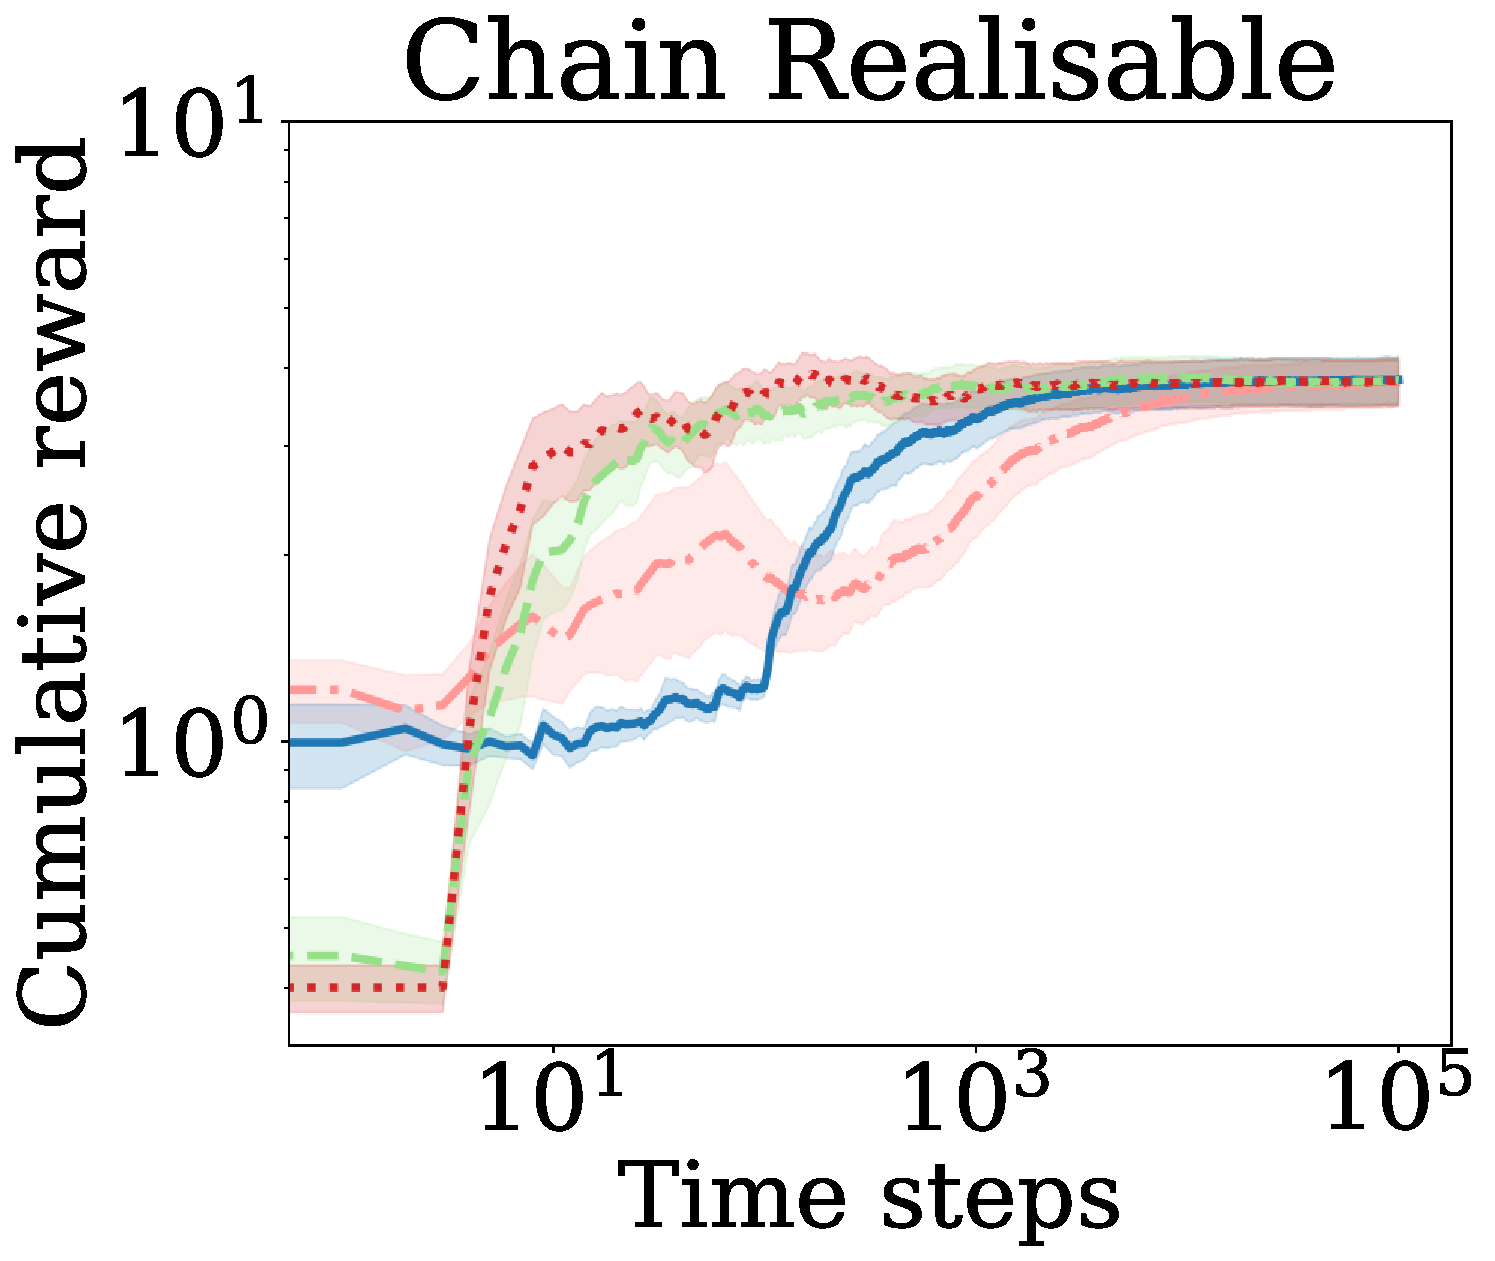
\includegraphics[width=0.3\textwidth]{YourThesis/papers/transfer-learning/img/chain_realisable.pdf}         
    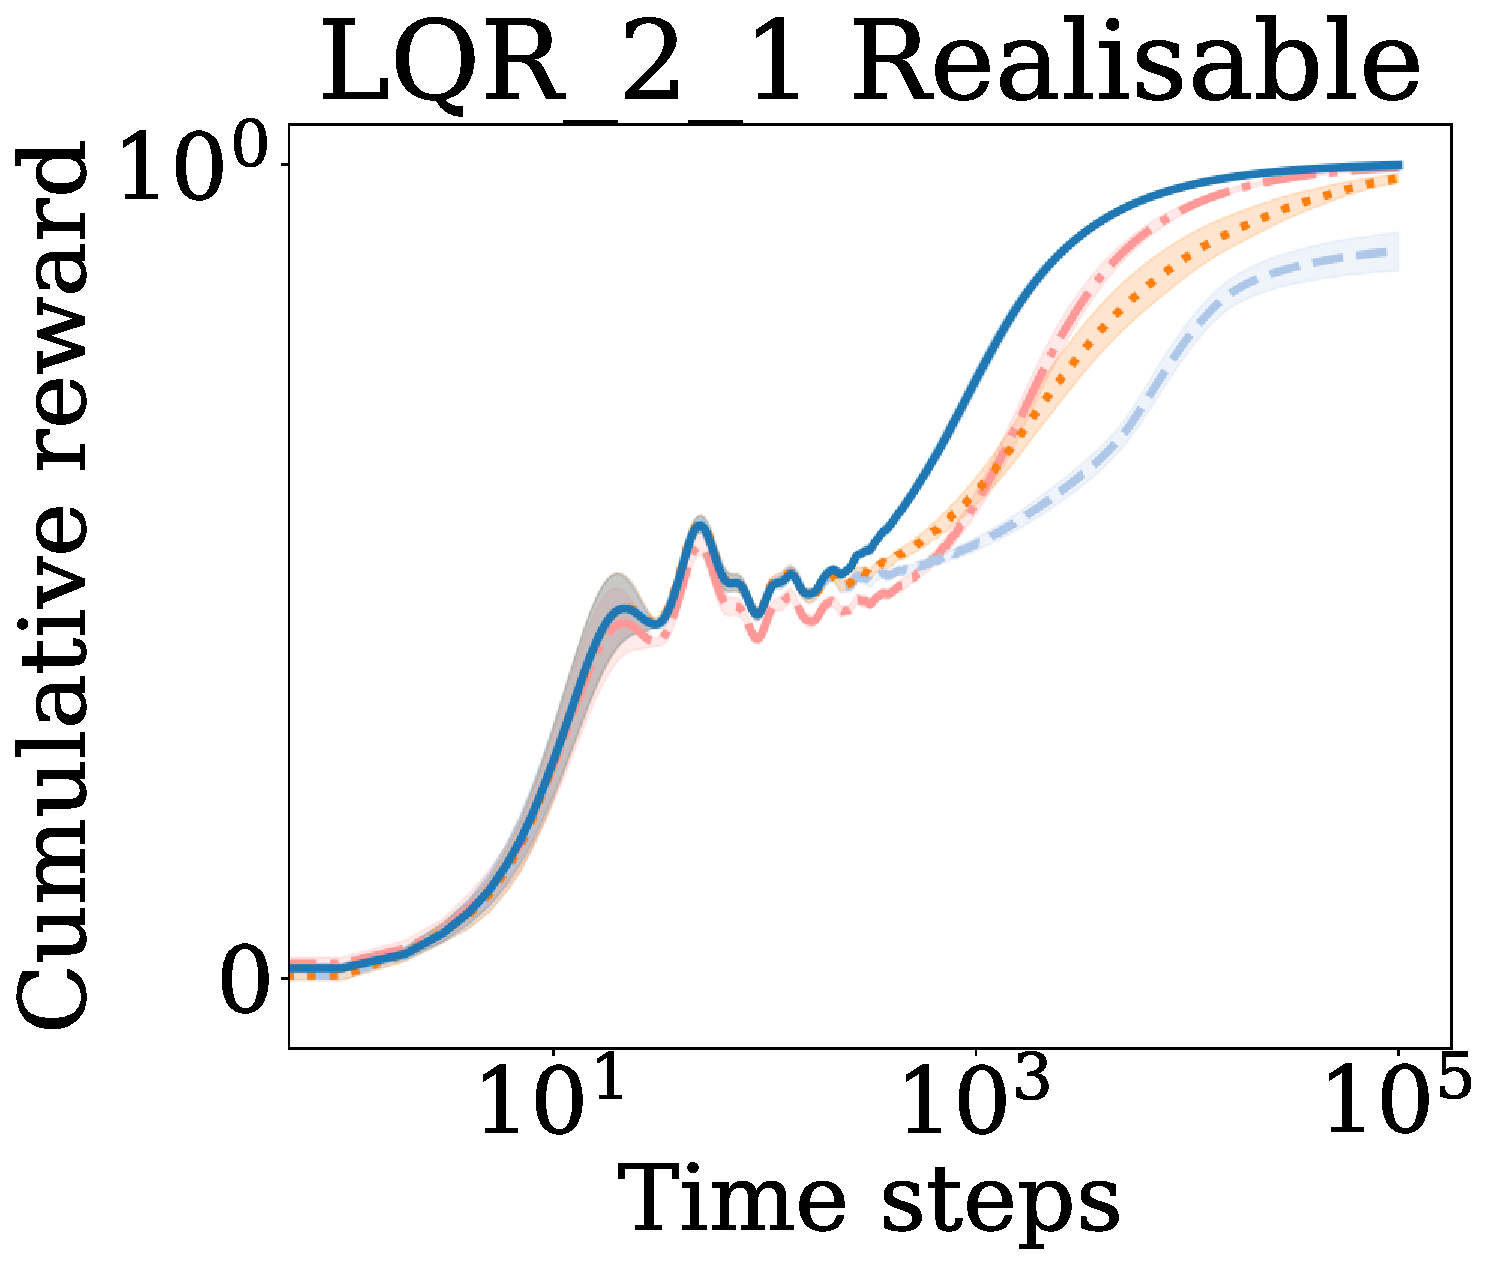
\includegraphics[width=0.45\textwidth]{YourThesis/papers/transfer-learning/img/lqr_2_1_realisable.pdf} 
    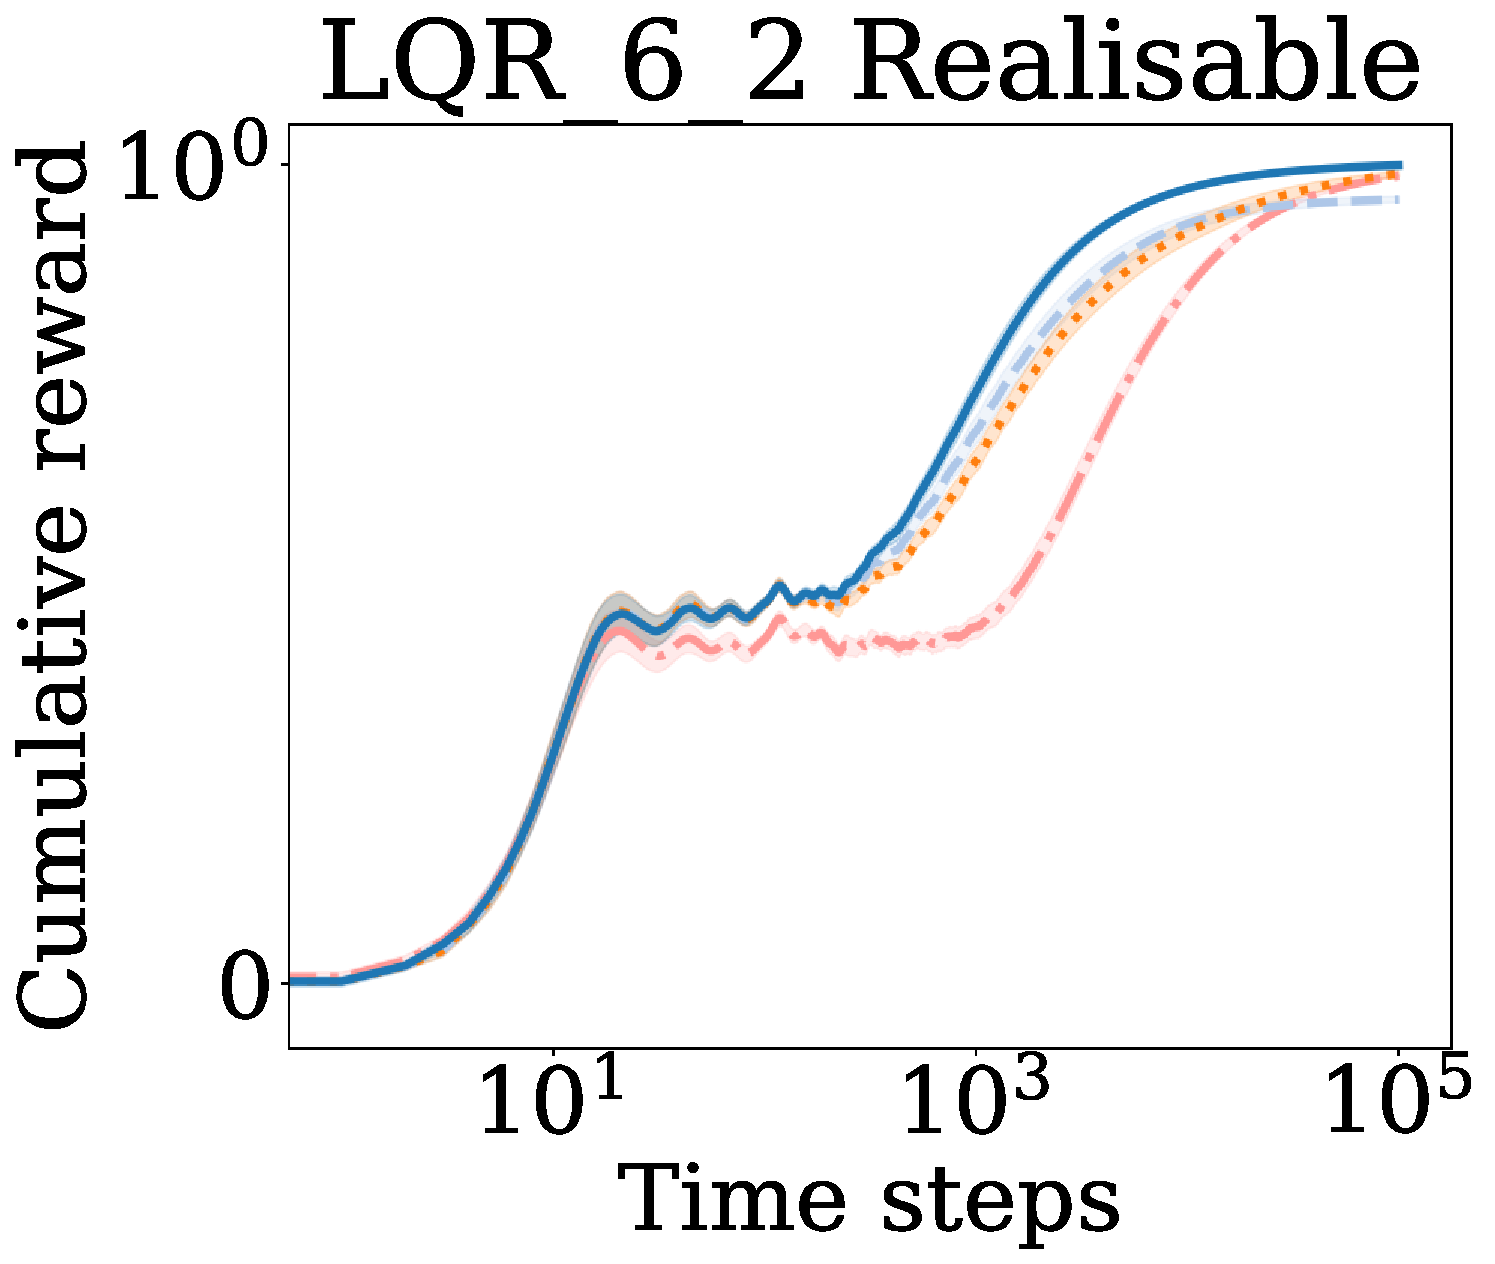
\includegraphics[width=0.45\textwidth]{YourThesis/papers/transfer-learning/img/lqr_6_2_realisable.pdf}\\
    % 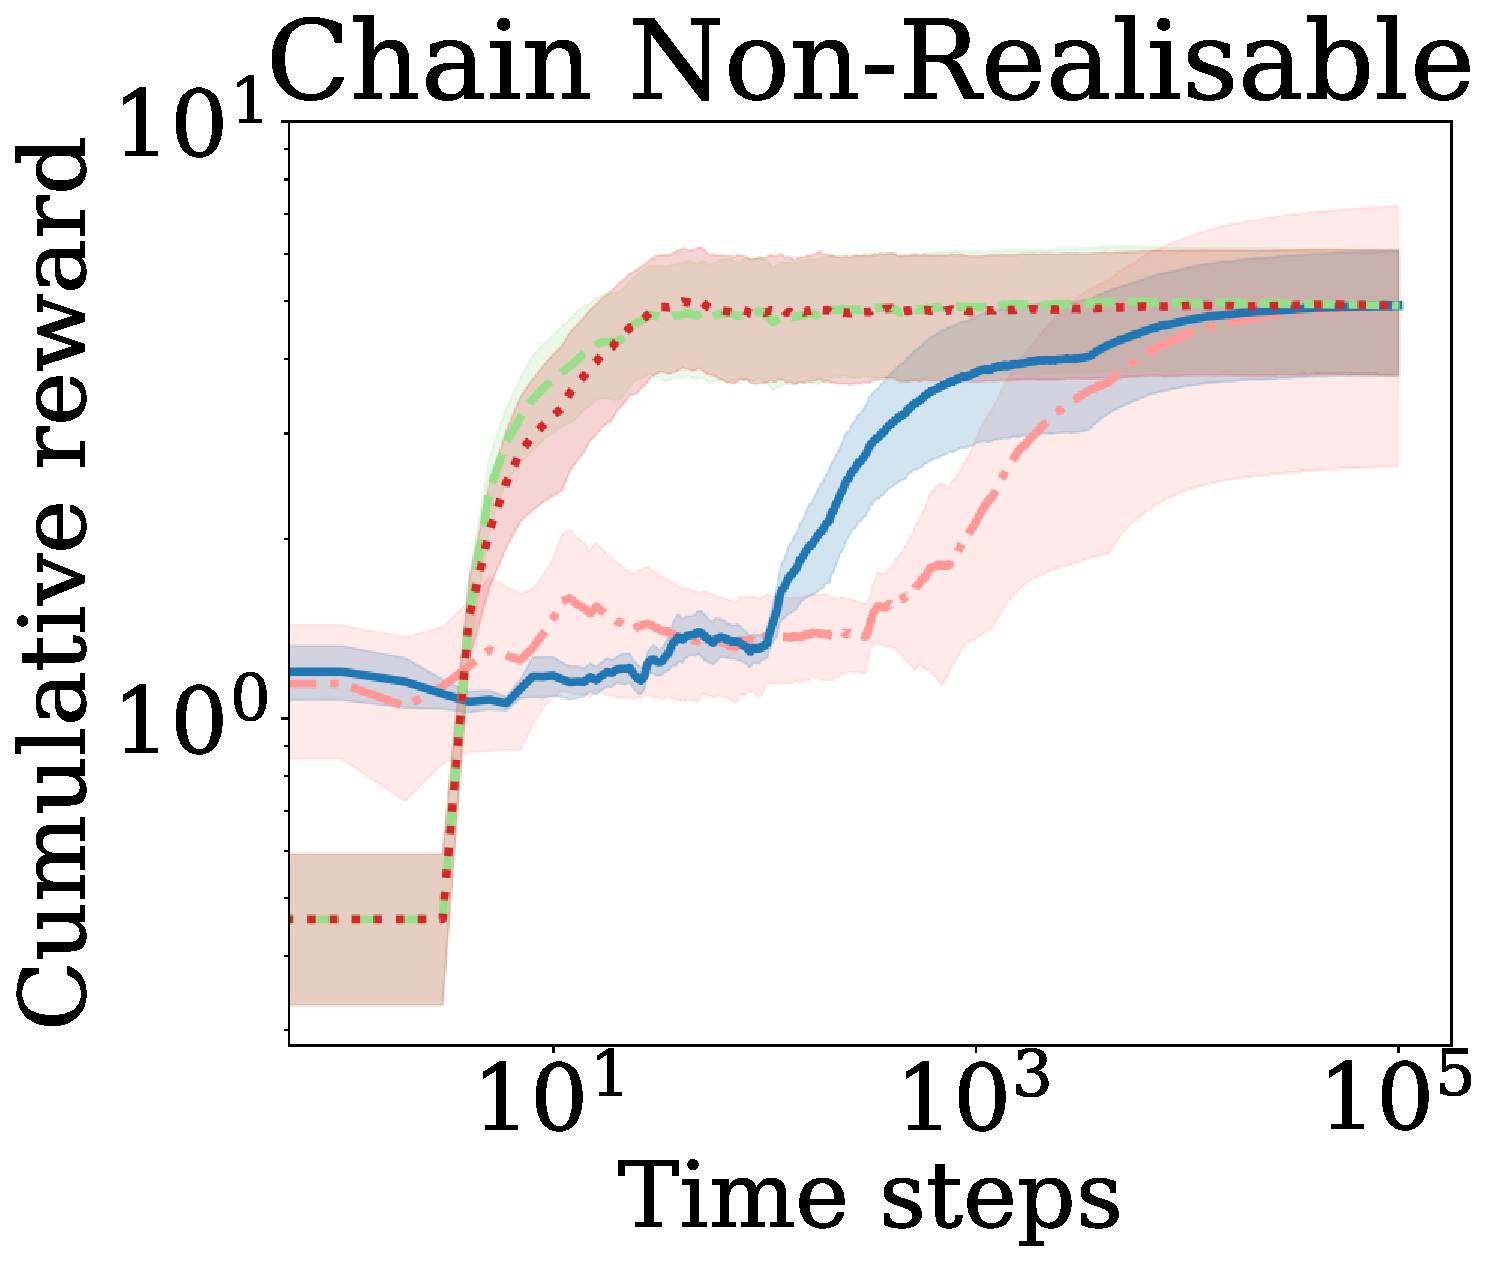
\includegraphics[width=0.3\textwidth]{img/chain_non_realisable.pdf}        
    % 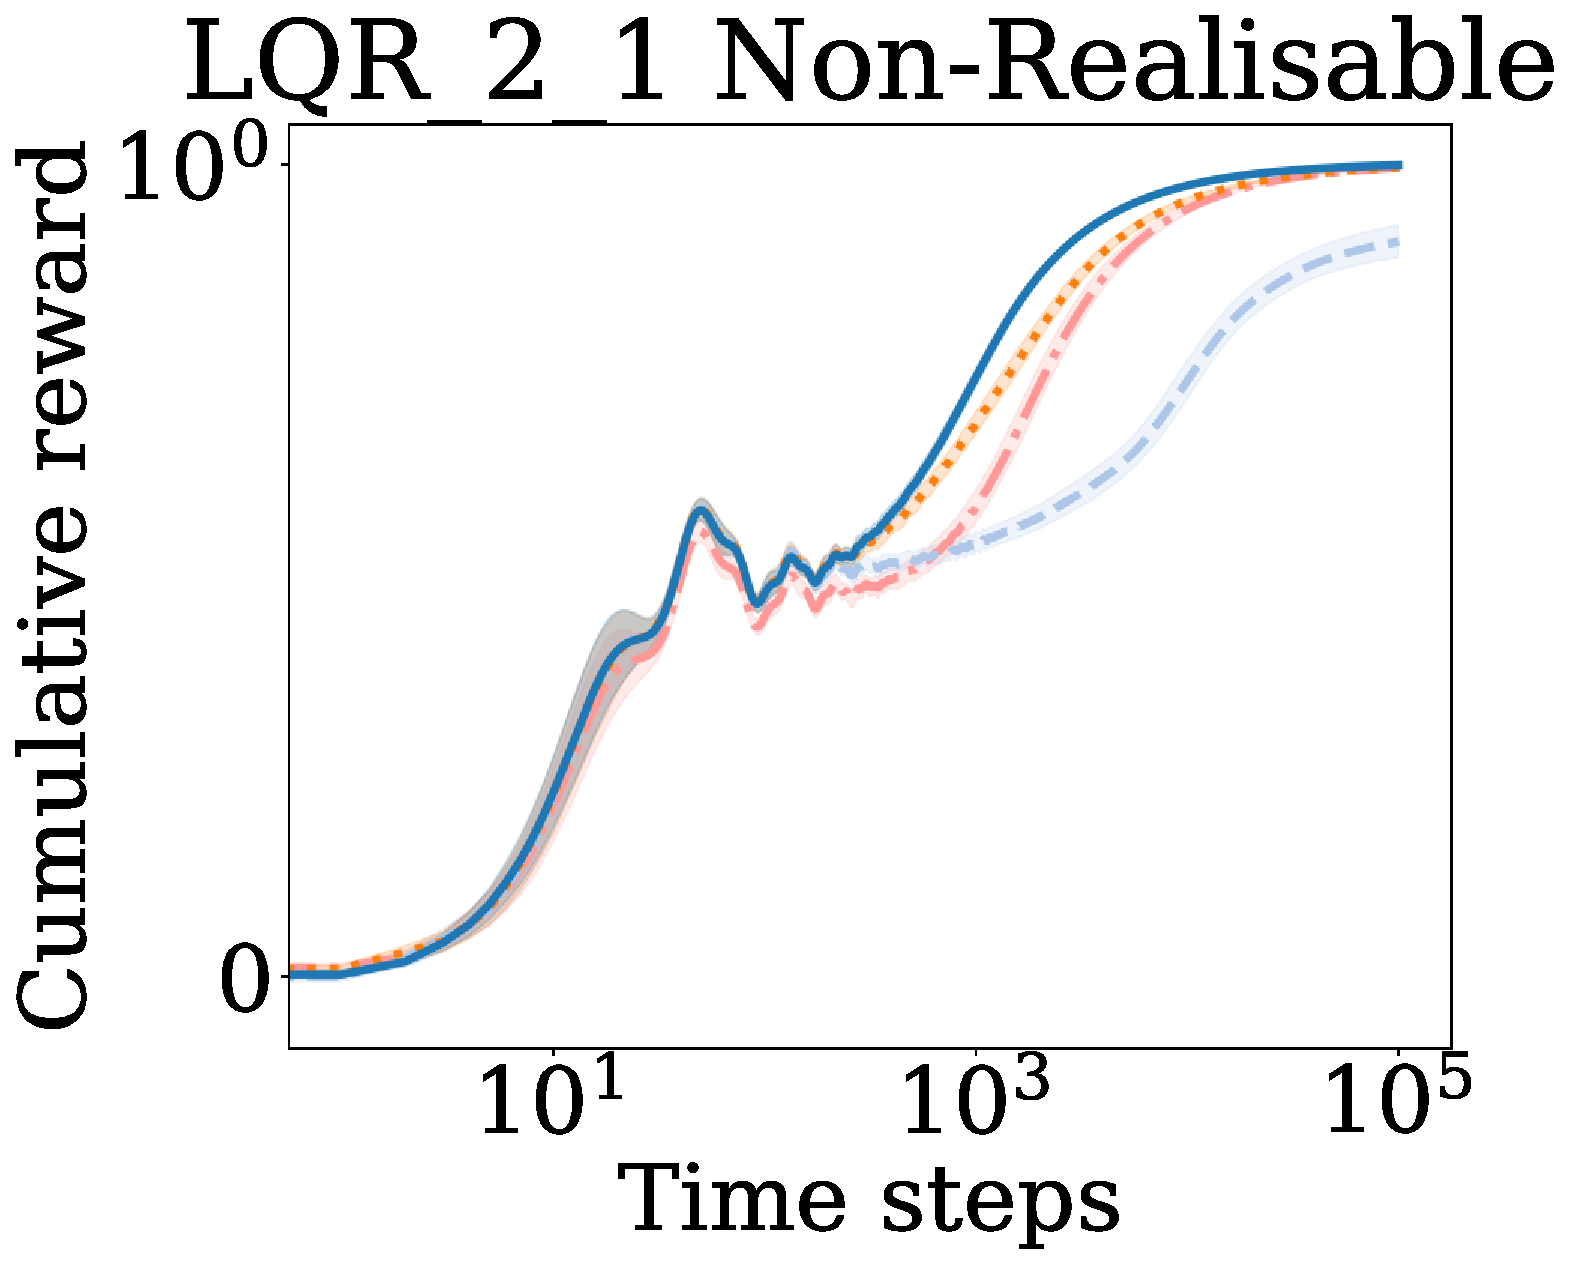
\includegraphics[width=0.3\textwidth]{img/lqr_2_1_non_realisable.pdf} 
    % 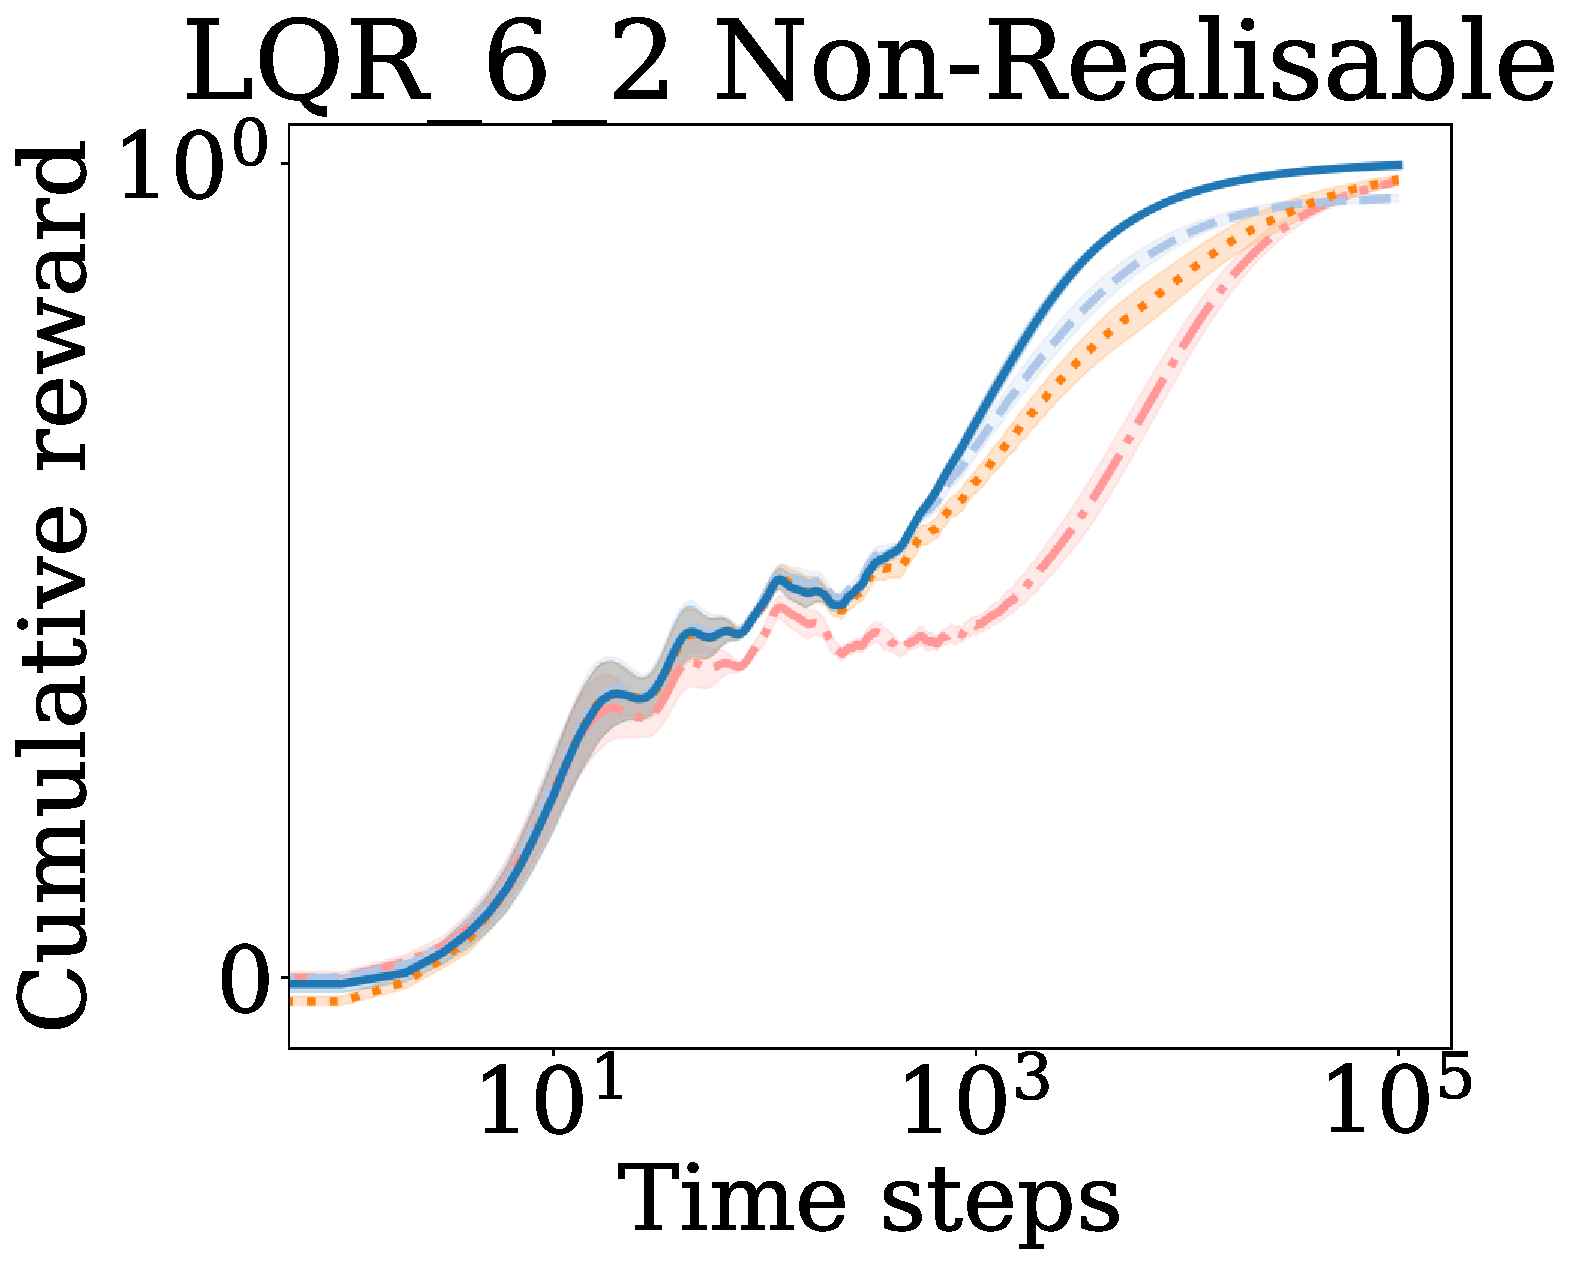
\includegraphics[width=0.3\textwidth]{img/lqr_6_2_non_realisable.pdf}\\
    
\includegraphics[width=\textwidth]{YourThesis/papers/transfer-learning/img/lqr_legend2.png}
    \caption{The average cumulative reward at every time step computed for two LQR tasks from Deepmind control suit. The shaded regions represent the standard error of the average cumulative reward at the time step.}\label{fig:thesis_full_results}%\vspace*{-1em}
\end{figure}

The results experiment are shown in Figure~\ref{fig:thesis_full_results}, where the performance metric is the average cumulative reward at each time step over $10^5$ time steps, with the shaded region representing the standard deviation. In these experiments, MLEMTRL demonstrates a clear advantage over all baselines in terms of learning speed improvement and asymptotic performance when compared to MT-SAC, but shows negligible differences in jumpstart improvements.

This shows that MLEMTRL is able to construct a model for an RL agent using a set of source models, provided that the target model is sufficiently similar to the source models.

% The experiments are done by varying the slippage parameter $p \in [0.00, 0.50]$ and the results are computed for each different setup of Chain from scratch. 
% In this experiment, the baseline algorithms MT-PPO and MT-PPO-TRL perform very well.
% This could partially be explained by PSRL and MLEMTRL not only having to learn the transition distribution but also the reward function. The value function transfer in the PPO-based baselines implicitly transfers not only the empirical transition model but also the reward function. We can see that MLEMTRL has improved learning speed compared to PSRL. 

% In Figure~\ref{fig:full_results}, the performance metric is the average cumulative reward at every time step, for $10^5$ time steps and the shaded region represents the standard deviation, where the statistics are computed over $10$ independent tasks. %\\


% How can we accurately construct a model using a set of source models for an RL agent deployed in the wild?
% Our answer to the first question is by adopting the Model Transfer Reinforcement Learning framework and weighting existing knowledge together with data from the novel task. We accomplished this by following a maximum likelihood-based approach. This has led to a novel algorithm, MLEMTRL, consisting of a model identification stage and a model-based planning stage.

% Does the constructed model allow us to perform efficient planning and yield improvements over learning from scratch? 
% The model allows generalizing to novel tasks, given that the tasks are similar enough to the existing task(s).
% We motivate the use of our framework in settings where an agent is to be deployed in a new domain that is similar to existing, known, domains.
% We verify the quick, near-optimal performance of the algorithm in the case where the new domain is similar and we prove worst-case performance bounds of the algorithm in both the realisable and non-realisable settings. 


